\section{Proofs}
\label{app:proofs}

\begin{proposition}[$\alpha_{\mathrm{eff}}$ monotonicity]
\label{prop:monotone}
$\alpha_{\mathrm{eff}}(b)$ is non-decreasing in $b$, and strictly increasing whenever the batch contains at least two samples with distinct $q$-values.
\end{proposition}

\begin{proof}[Proof of Proposition~\ref{prop:monotone}]
Let $w_i(b) = (1 - q_i)^b$, $W(b) = \sum_{j=1}^B w_j(b)$, and $\pi_i(b) = w_i(b) / W(b)$.
Then
\begin{equation*}
  \alpha_{\mathrm{eff}}(b) = \sum_{i=1}^{B} \pi_i(b)\, (1 - q_i).
\end{equation*}
Taking the derivative with respect to $b$:
\begin{align*}
  \frac{d\pi_i}{db}
  &= \pi_i \!\left(\frac{d \ln w_i}{db} - \frac{d \ln W}{db}\right) \\
  &= \pi_i \!\left(\ln(1{-}q_i) - \textstyle\sum_j \pi_j \ln(1{-}q_j)\right).
\end{align*}
Substituting,
\begin{align*}
  \frac{d\alpha_{\mathrm{eff}}}{db}
  &= \sum_i (1{-}q_i)\, \pi_i \!\left(\ln(1{-}q_i) - \mathbb{E}_{\pi}[\ln(1{-}q)]\right) \\
  &= \mathrm{Cov}_{\pi}\!\bigl(1{-}q_i,\, \ln(1{-}q_i)\bigr).
\end{align*}
Since $(1{-}q_i)$ and $\ln(1{-}q_i)$ are both increasing functions of $(1{-}q_i)$, they are positively associated, so the covariance is non-negative.
\end{proof}

\begin{proposition}[ESS monotonicity]
\label{prop:ess_mono}
$\mathrm{ESS}(b)$ is non-increasing in $b$, and strictly decreasing whenever the batch contains at least two samples with distinct $q$-values.
\end{proposition}

\begin{proof}
Write $\mathrm{ESS}(b) = 1 / \sum_i \pi_i(b)^2$, where $\pi_i(b) = w_i(b) / W(b)$.
The denominator $\sum_i \pi_i^2$ is the Herfindahl index $H$.
Differentiating $H$ with respect to $b$:
\begin{equation*}
  \frac{dH}{db} = 2 \sum_i \pi_i^2 \bigl(\ln(1{-}q_i) - \mathbb{E}_{\pi}[\ln(1{-}q)]\bigr).
\end{equation*}
Since $\pi_i \propto (1{-}q_i)^b$, larger $\pi_i$ implies larger $\ln(1{-}q_i)$; the $\pi^2$-weighted sum assigns greater mass to terms where $\ln(1{-}q_i) > \mathbb{E}_\pi[\ln(1{-}q)]$, so $dH/db \geq 0$, with strict inequality when at least two $q$-values differ.
Thus $H$ is non-decreasing and $\mathrm{ESS} = 1/H$ is non-increasing.
This is a standard property of exponential tilting~\citep{kish1965survey,owen2013mc}.
\end{proof}

\section{Algorithm Details}
\label{app:algorithm}

\begin{algorithm}[h]
\caption{Per-batch adaptive $b^{*}$ selection}
\label{alg:bstar}
\begin{algorithmic}[1]
\REQUIRE Batch scores $\{q_i\}_{i=1}^{B}$, threshold~$\tau$, ESS floor~$n_{\min}$, bound~$b_{\max}$, tol.~$\varepsilon$
\ENSURE Optimal sharpening exponent $b^{*}$
\IF{$\alpha_{\mathrm{eff}}(0) \geq \tau$}
  \STATE \textbf{return} $0$ \COMMENT{clean batch}
\ENDIF
\STATE $b_\tau \gets \textsc{Bisect}(\alpha_{\mathrm{eff}}(\cdot){=}\tau,\; [0, b_{\max}],\; \varepsilon)$
\IF{$\mathrm{ESS}(b_\tau) \geq n_{\min}$}
  \STATE \textbf{return} $b_\tau$ \COMMENT{$\alpha_{\mathrm{eff}}$-binding}
\ELSE
  \STATE $b_{\mathrm{ESS}} \gets \textsc{Bisect}(\mathrm{ESS}(\cdot){=}n_{\min},\; [0, b_{\max}],\; \varepsilon)$
  \STATE \textbf{return} $b_{\mathrm{ESS}}$ \COMMENT{ESS-binding}
\ENDIF
\end{algorithmic}
\end{algorithm}

\begin{figure}[h]
\centering
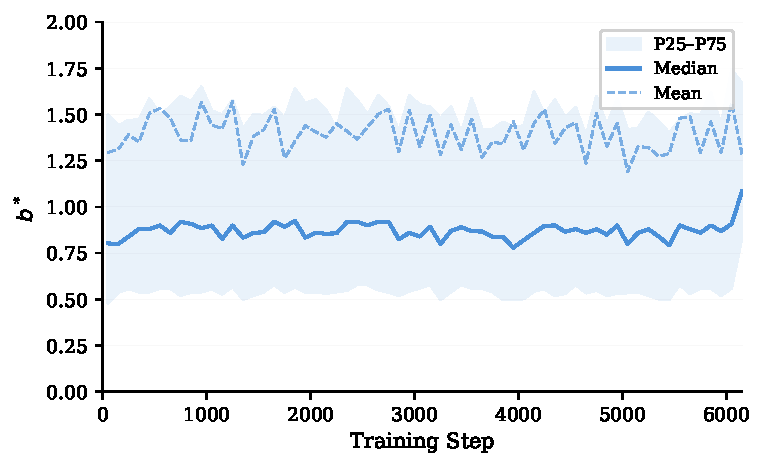
\includegraphics[width=\columnwidth]{bstar_trajectory_adaptive_fix}
\caption{Adaptive $\bstar$ trajectory over 6{,}103 training steps (seed\,42, $\rho{=}0.4$).
The exponent alternates between clean ($\bstar{=}0$), $\aeff$-binding, and ESS-binding regimes with no systematic drift, reflecting per-batch adaptation to local $q$-score composition.}
\label{fig:bstar_traj}
\end{figure}
We compute $\bstar$ at the micro-batch level ($B{=}4$) rather than the effective batch ($B{=}16$ after gradient accumulation) because $q$-score statistics exhibit sufficient variance within micro-batches: Spearman $r{=}0.699$ with the true real fraction, and at $B{=}16$ the adaptive advantage amplifies $3.0{\times}$ ($\Delta{=}{-}0.068{\pm}0.005$; \S\ref{sec:sensitivity}).

\section{Grid Search Details}
\label{app:grid}

Table~\ref{tab:grid_full} reports held-out PPL for all grid-$b$ values at $\rho = 0.4$ (seed\,42).

\begin{table}[h]
\centering
\small
\begin{tabular}{@{}cc@{}}
\toprule
$b$ & PPL $\downarrow$ \\
\midrule
0.1 & 17.657 \\
0.2 & 17.640 \\
0.3 & \textbf{17.640} \\
0.5 & 17.651 \\
1.0 & 17.692 \\
1.5 & 17.718 \\
2.0 & 17.741 \\
3.0 & 17.774 \\
5.0 & 17.818 \\
\bottomrule
\end{tabular}
\caption{Full grid search results ($\rho{=}0.4$, seed\,42).
$b \in [0.1, 0.5]$ forms a broad plateau (three-seed mean for $b{=}0.1$: $17.655 \pm 0.009$); $b{=}0.3$ is the post-hoc best.}
\label{tab:grid_full}
\end{table}

\section{Quality Threshold Sweep}
\label{app:tau_sweep}

\begin{table}[h]
\centering
\small
\resizebox{\columnwidth}{!}{%
\begin{tabular}{@{}ccccccc@{}}
\toprule
$\tau$ & Holdout $\downarrow$ & $\Delta_{\text{H}}$ & OWT $\downarrow$ & $\Delta_{\text{O}}$ & Wiki $\downarrow$ & $\Delta_{\text{W}}$ \\
\midrule
0.50 & 17.688 & $-$0.006 & -- & -- & -- & -- \\
0.60 & 17.681 & $-$0.013 & -- & -- & -- & -- \\
0.70$^\star$ & \textbf{17.674{\tiny$\pm$.006}} & $\boldsymbol{-}$\textbf{0.020} & \textbf{18.347{\tiny$\pm$.003}} & $\boldsymbol{-}$\textbf{0.028} & \textbf{15.330{\tiny$\pm$.015}} & $\boldsymbol{-}$\textbf{0.029} \\
0.80$^\star$ & 17.683{\tiny$\pm$.006} & $-$0.011 & 18.370{\tiny$\pm$.005} & $-$0.005 & 15.350 & $-$0.009 \\
0.90 & 17.712 & $+$0.018 & -- & -- & -- & -- \\
0.95 & 17.723 & $+$0.029 & -- & -- & -- & -- \\
\bottomrule
\end{tabular}}
\caption{Quality threshold sweep ($\nmin{=}2$, $\rho{=}0.4$).
$\Delta$ relative to 3-seed uniform baseline (Holdout 17.694, OWT 18.375, Wiki 15.359).
$^\star$\,$\tau{=}0.7$: 5-seed mean (SD from 5 seeds); $\tau{=}0.8$: 3 from-scratch seeds (Appendix~\ref{app:resume_artifact}). The 5-seed comparison in Table~\ref{tab:main} yields $\Delta{=}{-}0.023$.
Other values from single-seed exploratory sweep (seed\,42, holdout only).
$\tau{=}0.7$ achieves the lowest holdout and largest OOD gains ($|\Delta| \geq 0.028$); $\tau{=}0.8$'s OOD effect is smaller ($|\Delta| \leq 0.009$).}
\label{tab:tau}
\end{table}

\section{Batch-Adaptive $\tau$}
\label{app:batch_adaptive}

We tested a per-batch adaptive variant that clamps $\tau$ between 0.5 and the fixed threshold based on local $\aeff(0)$, allowing the quality floor to relax in batches with low estimated real fraction.
At both contamination levels ($\rho \in \{0.4, 0.6\}$), the adaptive variant did not outperform the fixed threshold (single-seed exploratory at each level), suggesting the quality constraint does not require adaptation to local contamination density.
This supports the ``two hyperparameters with good defaults'' characterization: neither $\tau$ nor $\nmin$ benefits from per-batch tuning.

\section{\texorpdfstring{$\tau$--$\rho$}{tau-rho} Rank Preservation}
\label{app:tau_rho}

Figure~\ref{fig:tau_rho_rank} shows the $\tau$--PPL relationship at two contamination levels.

\begin{figure}[h]
\centering
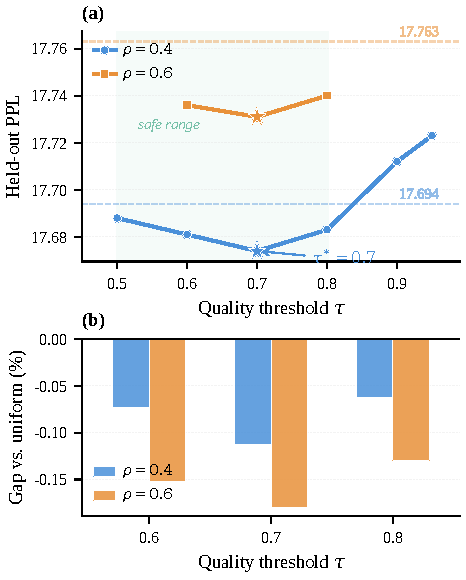
\includegraphics[width=\columnwidth]{tau_rho_rank_preservation}
\caption{(a) Held-out PPL as a function of quality threshold $\tau$ at $\rho \in \{0.4, 0.6\}$.
$\tau{=}0.7$ and $\tau{=}0.8$ yield comparable holdout PPL at $\rho{=}0.4$; at $\rho{=}0.6$, $\tau{=}0.7$ is statistically better (paired $t{=}{-}4.70$, $p{<}0.05$, 3 seeds, $\Delta{=}{-}0.005$). $\tau{=}0.7$ also achieves lower OOD perplexity at both levels ($\rho{=}0.6$: $\Delta_{\text{OWT}}{=}{-}0.014$, $\Delta_{\text{Wiki}}{=}{-}0.013$, 2 seeds).
(b) Normalized PPL gap relative to uniform at shared $\tau$ values.}
\label{fig:tau_rho_rank}
\end{figure}

\section{Hybrid and Threshold Comparison}
\label{app:hybrid}

Table~\ref{tab:hybrid} compares method families across contamination levels.
Table~\ref{tab:dr_threshold} shows D\&R sensitivity to the detection threshold at both full training length and epoch-matched settings.
Raw PPL traces a U-shaped curve with a minimum at $q{>}0.3$ (17.250, 3 seeds), but this curve conflates filtering quality with multi-epoch exposure: aggressive thresholds retain less data and repeat it more often.
Epoch-matched comparisons (rightmost column of Table~\ref{tab:dr_threshold}) remove the multi-epoch confound: the U-shape vanishes and PPL decreases monotonically, saturating near the adaptive $\bstar$ level at $q{\geq}0.5$.
Figure~\ref{fig:dr_dual_curve} visualizes the two curves.

\begin{table}[h]
\centering
\small
\begin{tabular}{@{}lcc@{}}
\toprule
\textbf{Method} & $\rho{=}0.4$ & $\rho{=}0.6$ \\
\midrule
Uniform & 17.694 & 17.766 \\
Adaptive $\bstar$ & 17.689 & 17.740 \\
Hybrid ($q{>}0.95$ + adaptive) & 17.514 & 17.530$^*$ \\
Detect \& Remove ($q{>}0.5$) & 17.285 & -- \\
Detect \& Remove ($q{>}0.3$) & 17.250 & -- \\
\bottomrule
\end{tabular}
\caption{Method comparison across contamination levels (seed\,42, $\tau{=}0.8$).
$^*$Hybrid at $\rho{=}0.6$ filters high-confidence synthetic ($q{>}0.95$), reducing effective $\rho$ to ${\approx}0.4$; PPL is not directly comparable to $\rho{=}0.6$ baselines.}
\label{tab:hybrid}
\end{table}

\begin{table}[h]
\centering
\small
\setlength{\tabcolsep}{3pt}
\begin{tabular}{@{}ccccc@{}}
\toprule
\textbf{Thresh.} & \textbf{Ret.\ \%} & \textbf{Epochs} & \textbf{Raw PPL} $\downarrow$ & \textbf{Ep.-matched} $\downarrow$ \\
\midrule
$q > 0.1$ & 15.0\% & ${\sim}$10.0 & 17.40 & 18.04 \\
$q > 0.2$ & ${\sim}$23\% & ${\sim}$5.0 & 17.27 & -- \\
$q > 0.3$ & 31.5\% & ${\sim}$3.2 & \textbf{17.250}$^\dagger$ & 17.74 \\
$q > 0.4$ & ${\sim}$38\% & ${\sim}$2.8 & 17.26 & -- \\
$q > 0.5$ & 41.4\% & ${\sim}$2.4 & 17.28 & 17.65 \\
$q > 0.6$ & ${\sim}$46\% & ${\sim}$1.7 & 17.30 & -- \\
$q > 0.7$ & 49.8\% & ${\sim}$2.0 & 17.32 & 17.62 \\
$q > 0.8$ & ${\sim}$56\% & ${\sim}$1.3 & 17.34 & -- \\
$q > 0.9$ & 61.6\% & ${\sim}$1.1 & 17.42 & 17.628 \\
\bottomrule
\end{tabular}
\caption{D\&R threshold sensitivity ($\rho{=}0.4$, seed\,42 unless noted).
Raw PPL traces a U-shaped curve (minimum at $q{>}0.3$); epoch-matched PPL (single content epoch) decreases monotonically and saturates near the adaptive $\bstar$ level (${\approx}$17.65) at $q{\geq}0.5$; the U-shape is thus a multi-epoch artifact.
$^\dagger$\,3-seed mean $17.250 \pm 0.001$.}
\label{tab:dr_threshold}
\end{table}

See Figure~\ref{fig:dr_dual_curve} (\S\ref{sec:main-results}) for the dual-curve visualization.

\section{Downstream Task Evaluation}
\label{app:downstream}

Table~\ref{tab:downstream} reports downstream benchmark accuracy for adaptive vs.\ uniform training at $\rho{=}0.4$ (seed\,42, Qwen3-0.6B).
Across multiple seeds, downstream differences are mixed in direction and uniformly within standard error, indicating that adaptive reweighting has no meaningful downstream impact.

\begin{table}[h]
\centering
\small
\resizebox{\columnwidth}{!}{%
\begin{tabular}{@{}llccc@{}}
\toprule
\textbf{Benchmark} & \textbf{Metric} & \textbf{Adaptive} & \textbf{Uniform} & $\boldsymbol{\Delta}$ \\
\midrule
\multicolumn{5}{@{}l}{\textit{Seed 42 (checkpoint resume)}} \\
ARC-Challenge & acc\_norm & 0.343 & 0.348 & $-$0.005 \\
ARC-Easy & acc & 0.650 & 0.657 & $-$0.007 \\
HellaSwag & acc\_norm & 0.479 & 0.484 & $-$0.005 \\
PIQA & acc & 0.687 & 0.686 & $+$0.001 \\
WinoGrande & acc & 0.578 & 0.586 & $-$0.008 \\
\midrule
\multicolumn{5}{@{}l}{\textit{From-scratch 2-seed mean (seeds 123, 456)}} \\
\multicolumn{3}{@{}l}{Mean $\Delta$ across 5 tasks} & & $+$0.001 \\
\multicolumn{3}{@{}l}{Direction} & \multicolumn{2}{c}{mixed (seed 123: 3/5$-$; seed 456: 3/5$+$)} \\
\bottomrule
\end{tabular}}
\caption{Downstream benchmarks (Qwen3-0.6B, $\rho{=}0.4$).
Seed\,42 used a checkpoint-resumed adaptive model; from-scratch seeds (123, 456) show mixed direction with mean $|\Delta| \leq 0.01$.
All differences within standard error ($\pm 0.01$).
Models use $\tau{=}0.8$; $\tau{=}0.7$ yields identical 3-seed means (0.5414).}
\label{tab:downstream}
\end{table}

\section{Higher Contamination Details}
\label{app:rho06}

Table~\ref{tab:rho06} reports results at $\rho{=}0.6$.
The full five-method ablation preserves the hierarchy from $\rho{=}0.4$ across all three seeds: Grid ${<}$ Adaptive ${<}$ Uniform ${\approx}$ ESS-only ${<}$ Random.

\begin{table}[h]
\centering
\small
\resizebox{\columnwidth}{!}{%
\begin{tabular}{@{}lcccc@{}}
\toprule
\textbf{Method} & \textbf{Seed 42} & \textbf{Seed 123} & \textbf{Seed 456} & \textbf{Mean} \\
\midrule
Grid ($b{=}0.3$)$^\ddagger$ & \textbf{17.634} & -- & -- & -- \\
Adaptive $\bstar$ & 17.735 & 17.727 & 17.732 & 17.731 $\pm$ .004 \\
Uniform           & 17.766 & 17.754 & 17.770 & 17.763 $\pm$ .008 \\
ESS-only          & 17.770 & 17.760 & 17.760 & 17.763 $\pm$ .006 \\
Random $\mathcal{U}(0,2)$ & 17.832 & 17.870 & 17.880 & 17.861 $\pm$ .025 \\
\bottomrule
\end{tabular}}
\caption{Results at $\rho{=}0.6$ (Qwen3-0.6B, $\nmin{=}2$).
Adaptive uses $\tau{=}0.7$ (consistent with main results); other methods are $\tau$-independent.
$^\ddagger$Post-hoc oracle; seed\,42 only.
Adaptive vs.\ Uniform: $\Delta{=}{-}0.032$, paired $t{=}{-}15.4$, $p{=}0.004$ (full precision; 3dp rounding yields $t{=}{-}9.95$, $p{=}0.010$).
ESS-only collapses onto Uniform (both $17.763$); Random ($17.861$) confirms detector signal is load-bearing.}
\label{tab:rho06}
\end{table}

The ESS-only/Uniform gap collapses from 0.043 at $\rho{=}0.4$ to 0.000 at $\rho{=}0.6$ (three-seed means: both $17.763$); ESS binding rises to ${\sim}$49\% of batches (from ${\sim}$43\% at $\rho{=}0.4$), and the constraints become nearly balanced rather than $\aeff$-dominant.
The adaptive method maintains its advantage ($\Delta{=}{-}0.032$, consistent across seeds) through the $\aeff$ quality constraint, which operates independently of the ESS ceiling.
Random reweighting ($17.861 \pm 0.025$) is substantially worse than Uniform, with the highest cross-seed variance; uninformed weights add noise without corrective signal.
The Adaptive-vs-Grid gap is 0.054 at $\rho{=}0.4$ (mean-to-mean, consistent with Table~\ref{tab:aux}) and 0.097 at $\rho{=}0.6$ (adaptive 3-seed mean vs.\ grid seed\,42; the $\rho{=}0.6$ grid result is preliminary and may not generalize across seeds).

\section{\texorpdfstring{$\alpha_{\mathrm{eff}}$}{alpha-eff} Proxy Validation}
\label{app:alpha_validation}

Table~\ref{tab:alpha_corr} reports the correlation between $\aeff(0)$ (the detector-based proxy at $b{=}0$) and the true batch-level real fraction $\alpha_{\mathrm{true}}$, computed over all training batches at $\rho{=}0.4$ (seed\,42).

\begin{table}[h]
\centering
\small
\begin{tabular}{@{}ccccc@{}}
\toprule
$B$ & Pearson $r$ & Spearman $r$ & MAE$\downarrow$ & Bias \\
\midrule
4  & 0.706 & 0.699 & 0.114 & $-$0.029 \\
8  & 0.697 & 0.683 & 0.097 & $-$0.027 \\
16 & 0.707 & 0.691 & 0.075 & $-$0.031 \\
\bottomrule
\end{tabular}
\caption{Correlation between $\aeff(0)$ and true batch-level real fraction across batch sizes ($\rho{=}0.4$, seed\,42).
Values use a binarized proxy $\hat{r}_i = \mathbf{1}[q_i \leq 0.5]$ for discrete comparison; the continuous formulation used during training (\S\ref{sec:method}) achieves $r \approx 0.77$--$0.79$ depending on batch size.
The consistent negative bias (${\approx}{-}0.03$) indicates that $\aeff$ slightly underestimates the true real fraction, biasing the method toward conservative intervention.}
\label{tab:alpha_corr}
\end{table}

Mean absolute error (MAE) decreases with batch size (0.114 $\to$ 0.075) as expected from averaging, but the rank-order information that drives $\bstar$ selection is already well-captured at $B{=}4$.

\paragraph{Cross-seed stability.}
Table~\ref{tab:alpha_corr_perseed} reports the correlation between $\aeff$ and the batch mean $q$-score ($\bar{q}$, computed from known labels) across all three seeds.

\begin{table}[h]
\centering
\small
\begin{tabular}{@{}cccc@{}}
\toprule
\textbf{Seed} & Pearson $r(\aeff, \bar{q})$ & Spearman $\rho_s$ & $\bstar{=}0$ (\%) \\
\midrule
42  & 0.8019 & 0.8761 & 5.8 \\
123 & 0.7994 & 0.8692 & 5.7 \\
456 & 0.8006 & 0.8749 & 5.9 \\
\midrule
\textbf{Spread} & 0.0025 & 0.0069 & 0.2 \\
\bottomrule
\end{tabular}
\caption{Per-seed $\aeff$--$\bar{q}$ correlation ($\rho{=}0.4$, $B{=}4$).
Cross-seed spread is $<$0.003 for Pearson $r$ and $<$0.007 for Spearman $\rho_s$, indicating stable proxy fidelity across random seeds.
$r(\aeff, \bar{q}) = 0.80$ measures the proxy's fidelity to batch composition; the ground-truth correlation $r(\aeff, \text{true real fraction}) \approx 0.79$ (\S\ref{sec:discussion}) is slightly lower due to detector noise.
The per-seed table demonstrates cross-seed stability rather than superseding the ground-truth estimate.}
\label{tab:alpha_corr_perseed}
\end{table}

\section{Detector Comparison}
\label{app:detector}

See Figure~\ref{fig:overview}b (\S\ref{sec:robustness}) for the detector requirements visualization.

Table~\ref{tab:detector} compares three detector families for adaptive reweighting.
The discriminative TF-IDF+LR detector (ECE\,=\,0.048) produces the only improvement over uniform.
The TF-IDF vs.\ GPT-2 contrast (comparable AUC: 0.94 vs.\ 0.91, but $2.7{\times}$ ECE gap: 0.048 vs.\ 0.131) isolates calibration as an empirically observed requirement; however, N-gram's better ECE (0.069) does not compensate for its low AUC (0.73); both sufficient discrimination and good calibration are jointly necessary in our setting.
TF-IDF+LR's $q$-scores have reliable probabilistic semantics, so the $\aeff$ proxy accurately tracks batch quality.
Generative detectors assign high $q$-scores to fluent, predictable human text (false positives concentrated among high-quality samples), systematically inflating $\aeff$ for clean batches and deflating it for contaminated ones, which inverts the minimum-intervention logic.

\begin{table}[h]
\centering
\small
\resizebox{\columnwidth}{!}{%
\begin{tabular}{@{}llccccc@{}}
\toprule
\textbf{Detector} & \textbf{Type} & \textbf{AUC} & \textbf{ECE} & \textbf{Mean PPL} & $\boldsymbol{\Delta}$ \\
\midrule
TF-IDF+LR & Discriminative & 0.94 & 0.048 & 17.650{\tiny$\pm$.010} & $-$0.044 \\
GPT-2 PPL & Generative & 0.91 & 0.131 & 17.792{\tiny$\pm$.005} & $+$0.098 \\
N-gram PPL & Generative & 0.73 & 0.069 & 17.823{\tiny$\pm$.003} & $+$0.129 \\
\bottomrule
\end{tabular}}
\caption{Detector comparison for adaptive reweighting ($\rho{=}0.4$, $\tau{=}0.8$, 3 seeds).
Uniform baseline PPL\,=\,17.694.
$\Delta$ = Adaptive $-$ Uniform (negative is better).
TF-IDF+LR calibrated via temperature scaling.
The $\tau$ confound is conservative: TF-IDF+LR at $\tau{=}0.7$ achieves 17.674 (Table~\ref{tab:main}).}
\label{tab:detector}
\end{table}

\section{Detector and Synthetic Data Details}
\label{app:detector_details}

\paragraph{TF-IDF+LR detector.}
TF-IDF features (unigrams + bigrams, max 50{,}000 features, sublinear TF) fed to Logistic Regression (C\,=\,1.0, L2 penalty, solver\,=\,lbfgs, max\_iter\,=\,100).
Trained on a held-out labeled split (10K documents per class).
Post-hoc temperature scaling applied when uncalibrated ECE exceeds 0.05: a scalar $T$ is searched via \texttt{scipy.optimize.minimize\_scalar} over $[0.1, 10.0]$ on a 20\% stratified validation split, yielding $T{=}0.204$ (ECE reduced from 0.12 to 0.048).
The detector is selected automatically from six configurations as the first satisfying AUC $\in [0.85, 0.98]$ and mid-range score ratio $\geq 5\%$.

\paragraph{Synthetic data generation.}
Continuations generated with Qwen3-0.6B (self-generation) using nucleus sampling ($p{=}0.95$, $T{=}0.8$), producing up to 384 tokens per continuation from a 128-token prefix prompt (512 total), targeting ${\sim}$100M synthetic tokens.
Source prompts are the first 128 tokens of randomly sampled FineWeb documents, used as prefix continuations.
Injected at token-level ratio $\rho$ via uniform random mixing across the training corpus.

\section{Low Contamination Analysis}
\label{app:rho02}

At $\rho{=}0.2$, the adaptive method degrades by $+$0.046 PPL relative to uniform (0.26\% relative, seed\,42).
The detector's mean $q$-score at this contamination level is 0.393 (vs.\ 0.487 at $\rho{=}0.4$), indicating that many clean samples receive moderate $q$-scores, blurring the provenance signal.
The regime decomposition reveals 13.7\% clean batches ($\bstar{=}0$), 60.1\% $\aeff$-binding, and 26.3\% ESS-binding, with mean $\bstar{=}1.735$ in reweighted batches.
The high $\aeff$-binding rate (60.1\% vs.\ ${\sim}$50\% at $\rho{=}0.4$) means the method actively intervenes rather than defaulting to $\bstar{=}0$, but the unreliable signal causes it to suppress useful training data.
This is consistent with the generative detector failures: when $q$-scores do not reliably separate provenance, the minimum intervention framework amplifies the error rather than correcting it.
The effective range of the method is $\rho \geq 0.4$ with $\tau \in [0.7, 0.8]$ (\S\ref{sec:sensitivity}); lower $\tau$ values may extend the range but have not been tested at $\rho{=}0.2$.

\section{Cross-Model Transfer}
\label{app:cross_model}

Table~\ref{tab:cross_model} reports a single exploratory run with Llama-3.2-3B as a cross-generator (synthetic data generated by Llama, training on Qwen3-0.6B); this does not establish generality.
Results are mixed: MMLU improves while HellaSwag slightly degrades, consistent with the pattern observed in Qwen3-1.7B downstream evaluation (\S\ref{sec:robustness}).
Perplexity comparison omitted due to inconsistent evaluation configurations; checkpoints were not retained for re-evaluation.

\begin{table}[h]
\centering
\small
\resizebox{\columnwidth}{!}{%
\begin{tabular}{@{}lccc@{}}
\toprule
\textbf{Metric} & \textbf{Uniform} & \textbf{Adaptive} & $\boldsymbol{\Delta}$ \\
\midrule
MMLU (5-shot) & 51.85\% $\pm$ .41 & 53.42\% $\pm$ .41 & $+$1.57pp \\
HellaSwag (10-shot, acc\_norm) & 73.08\% $\pm$ .44 & 72.49\% $\pm$ .45 & $-$0.59pp \\
\bottomrule
\end{tabular}}
\caption{Cross-model transfer: Llama-3.2-3B generator, Qwen3-0.6B trainer ($\rho{=}0.4$, single seed).
Mixed results reflect evaluation-set distribution sensitivity rather than consistent quality differences.}
\label{tab:cross_model}
\end{table}

\section{Checkpoint Resume Artifact}
\label{app:resume_artifact}

The checkpoint-resume artifact described here affected early $\tau{=}0.8$ experiments only.
All results in Tables~\ref{tab:main}--\ref{tab:epoch_match} use independent from-scratch training ($\tau{=}0.7$; Table~\ref{tab:main} Adaptive/Uniform: five seeds, others: three seeds).

The adaptive model for seed\,42 in early $\tau{=}0.8$ runs was trained with a checkpoint-resumed run whose first ${\sim}$1{,}000 steps used different hyperparameters (learning rate warmup, gradient accumulation configuration) than seeds 123 and 456, which were trained from scratch.
The resume artifact inflates the in-distribution effect ($\Delta{=}{-}0.041$ resume vs.\ $\Delta{=}{-}0.005$ from-scratch at $\tau{=}0.8$) and reverses the out-of-distribution direction:

\begin{center}
\small
\begin{tabular}{@{}lccc@{}}
\toprule
\textbf{Domain} & \textbf{Resume} & \textbf{From-scratch} & \textbf{Dir.} \\
\midrule
FineWeb (in-dist) & $-$0.041 & $-$0.005 & same \\
OpenWebText (OOD) & $+$0.058 & $-$0.005 & reversed \\
Wikipedia (OOD)   & $+$0.137 & $-$0.009 & reversed \\
\bottomrule
\end{tabular}\\[2pt]
{\scriptsize $\Delta$ relative to from-scratch uniform (Table~\ref{tab:tau}). Resume: seed\,42 original checkpoint. From-scratch: clean replication run.}
\end{center}

The resume model showed apparent distribution matching (OOD degradation), which was the basis for the ``distribution matching'' finding in earlier analyses.
From-scratch retraining eliminates this pattern: all three evaluation domains show small, directionally consistent improvements, providing no evidence of distribution matching.
This underscores the importance of controlling for training artifacts when interpreting small effect sizes across evaluation domains.

\section{Additional Contamination Rate}
\label{app:rho03}

To probe the boundary between the degradation regime ($\rho{=}0.2$, $\Delta{=}{+}0.046$) and the improvement regime ($\rho{=}0.4$, $\Delta{=}{-}0.023$), we run adaptive $\bstar$ and uniform baselines at $\rho{=}0.3$ using the same experimental setup as the main experiments (Qwen3-0.6B, 132M FineWeb tokens, $\tau{=}0.7$, $\nmin{=}2$).

\begin{table}[h]
\centering
\small
\begin{tabular}{@{}lcccc@{}}
\toprule
\textbf{Method} & \textbf{Seed} & \textbf{FineWeb} $\downarrow$ & \textbf{OWT} $\downarrow$ & \textbf{Wiki} $\downarrow$ \\
\midrule
Uniform          & 42  & 17.422 & 18.113 & 15.204 \\
Adaptive $\bstar$ & 42  & 17.422 & 18.123 & 15.172 \\
\midrule
Uniform          & 123 & 17.433 & 18.126 & 15.204 \\
Adaptive $\bstar$ & 123 & 17.435 & 18.148 & 15.165 \\
\midrule
Uniform          & 456 & 17.419 & -- & -- \\
Adaptive $\bstar$ & 456 & 17.424 & -- & -- \\
\midrule
$\Delta$ (3-seed mean) & --  & $+$0.002 & -- & -- \\
\bottomrule
\end{tabular}
\caption{Results at $\rho{=}0.3$ (Qwen3-0.6B, 3 seeds).
Holdout $\Delta{=}{+}0.002$ ($t(2){=}1.60$, $p{=}0.25$, non-significant); OOD available for seeds 42 and 123 only, mixed in direction.}
\label{tab:rho03}
\end{table}

The holdout difference is effectively zero ($\Delta{=}{+}0.002$, $t(2){=}1.60$, $p{=}0.25$, non-significant), placing the transition boundary between the degradation regime ($\rho{=}0.2$, $\Delta{=}{+}0.046$) and the improvement regime ($\rho{=}0.4$, $\Delta{=}{-}0.023$) within $[0.3, 0.4]$ (Figure~\ref{fig:delta_vs_rho}).

At $\rho{=}0.3$, 28\% of micro-batches have $\bstar{=}0$ (clean, no intervention), compared to ${\sim}$6\% at $\rho{=}0.4$; the low intervention frequency explains why the method neither helps nor harms.
The progression across contamination levels ($\rho{=}0.2$ harmful, $+$0.046; $\rho{=}0.3$ neutral, $+$0.002; $\rho{=}0.4$ beneficial, $-$0.023) shows a graceful transition rather than abrupt failure, consistent with the detector's signal-to-noise ratio gradually crossing the threshold needed for reliable $\aeff$ estimation.

\section{Statistical Power Analysis}
\label{app:power}

The adaptive-vs-uniform comparison at $\rho{=}0.4$ has Cohen's $d = \bar{\Delta}/\mathrm{SD}_{\Delta} = 0.023/0.006 = 3.83$ (5 seeds, paired).
A one-sided paired $t$-test at $\alpha{=}0.05$ with $d{=}3.83$ and $N{=}5$ achieves statistical power ${>}0.99$ (noncentrality $\lambda = d\sqrt{N} = 8.56$, $t_{0.05,4} = 2.13$), indicating that $N{=}5$ is more than adequate to detect an effect of this magnitude.

The low cross-seed variance ($\sigma{=}0.006$) reflects the experimental design: seeds affect only parameter initialization, not data order (the dataloader is deterministic), so the primary stochastic axis is initialization noise at 0.6B scale.
The uniform baseline exhibits comparable variance ($\sigma{=}0.008$); the low dispersion is a property of the experimental setting rather than a method artifact.

We apply Bonferroni--Holm correction for $k{=}9$ family-wise comparisons (six reweighting methods $\times$ one contamination level, plus three additional $\rho$ levels).
After correction, $p_{\mathrm{BH}}{=}0.011$ at $\rho{=}0.4$, reaching conventional significance at $\alpha{=}0.05$.
At $\rho{=}0.6$ (3 seeds), $p_{\mathrm{BH}}{=}0.064$; the family includes structurally heterogeneous tests (different methods, different $\rho$), which makes Bonferroni--Holm conservative.
The uncorrected $p$-values ($0.0012$ and $0.010$ respectively), directional consistency across all seeds, and the dose-response pattern across $\rho$ levels collectively support a real effect.

\section{Supplementary Analyses Summary}
\label{app:summary}

\begin{table}[h]
\centering
\small
\setlength{\tabcolsep}{3pt}
\resizebox{\columnwidth}{!}{%
\begin{tabular}{@{}lll@{}}
\toprule
\textbf{Analysis} & \textbf{Key result} & \textbf{App.} \\
\midrule
Downstream tasks & No gain (5 benchmarks, $|\Delta|\leq 0.01$) & \ref{app:downstream} \\
Cross-model (Llama) & Mixed (MMLU $+$1.6, HellaSwag $-$0.6) & \ref{app:cross_model} \\
$\tau$ sweep & $[0.5,0.8]$ all improve; $\tau{>}0.8$ degrades & \ref{app:tau_sweep} \\
$\rho{=}0.3$ boundary & $\Delta{=}{+}0.002$ (neutral, 3 seeds) & \ref{app:rho03} \\
Statistical power & Cohen's $d{=}3.83$, power ${>}0.99$ at $N{=}5$ & \ref{app:power} \\
\bottomrule
\end{tabular}}
\caption{Summary of supplementary analyses.}
\label{tab:appendix_summary}
\end{table}

\section{Use of AI Assistance}

We used Claude for coding, code drafting, debugging, and language polishing.

